\section{Measurement system}
The purpose of the measurements is to test the algorithm real performance in outdoor conditions. The algorithm is first test in a controlled environment and in a second time to it put to the test in more challenging environements to find its limitation. A wide range of sources and environments are selected and tested in the following section.

\subsection{Microphone array and acquisition system}

A prototype microphone array is used to record sound on the field and in the anechoic chamber. 4 Brüel \& Kjaær microphones type 4935 are placed in a tetrahedral configuration as drawn in picture \ref{fig:micarraypic}. The height of the array can be ajusted by translating the middle vertical rode. The 4 microphones are omnidirectional and mounted on the array in a vertical position.
The Brüel \& Kjaær pulse acquisition system is used along with its own software suite. The module Type 3050-A-060 is the main interface of the chain and microphones are plugged throught BNC connection. During measurements outside, wind protection are also mounted on the microphones. The software records wave files with a sampling rate of 131072Hz which is the maximum sampling rate available.

\begin{figure}[H]
    \centering
    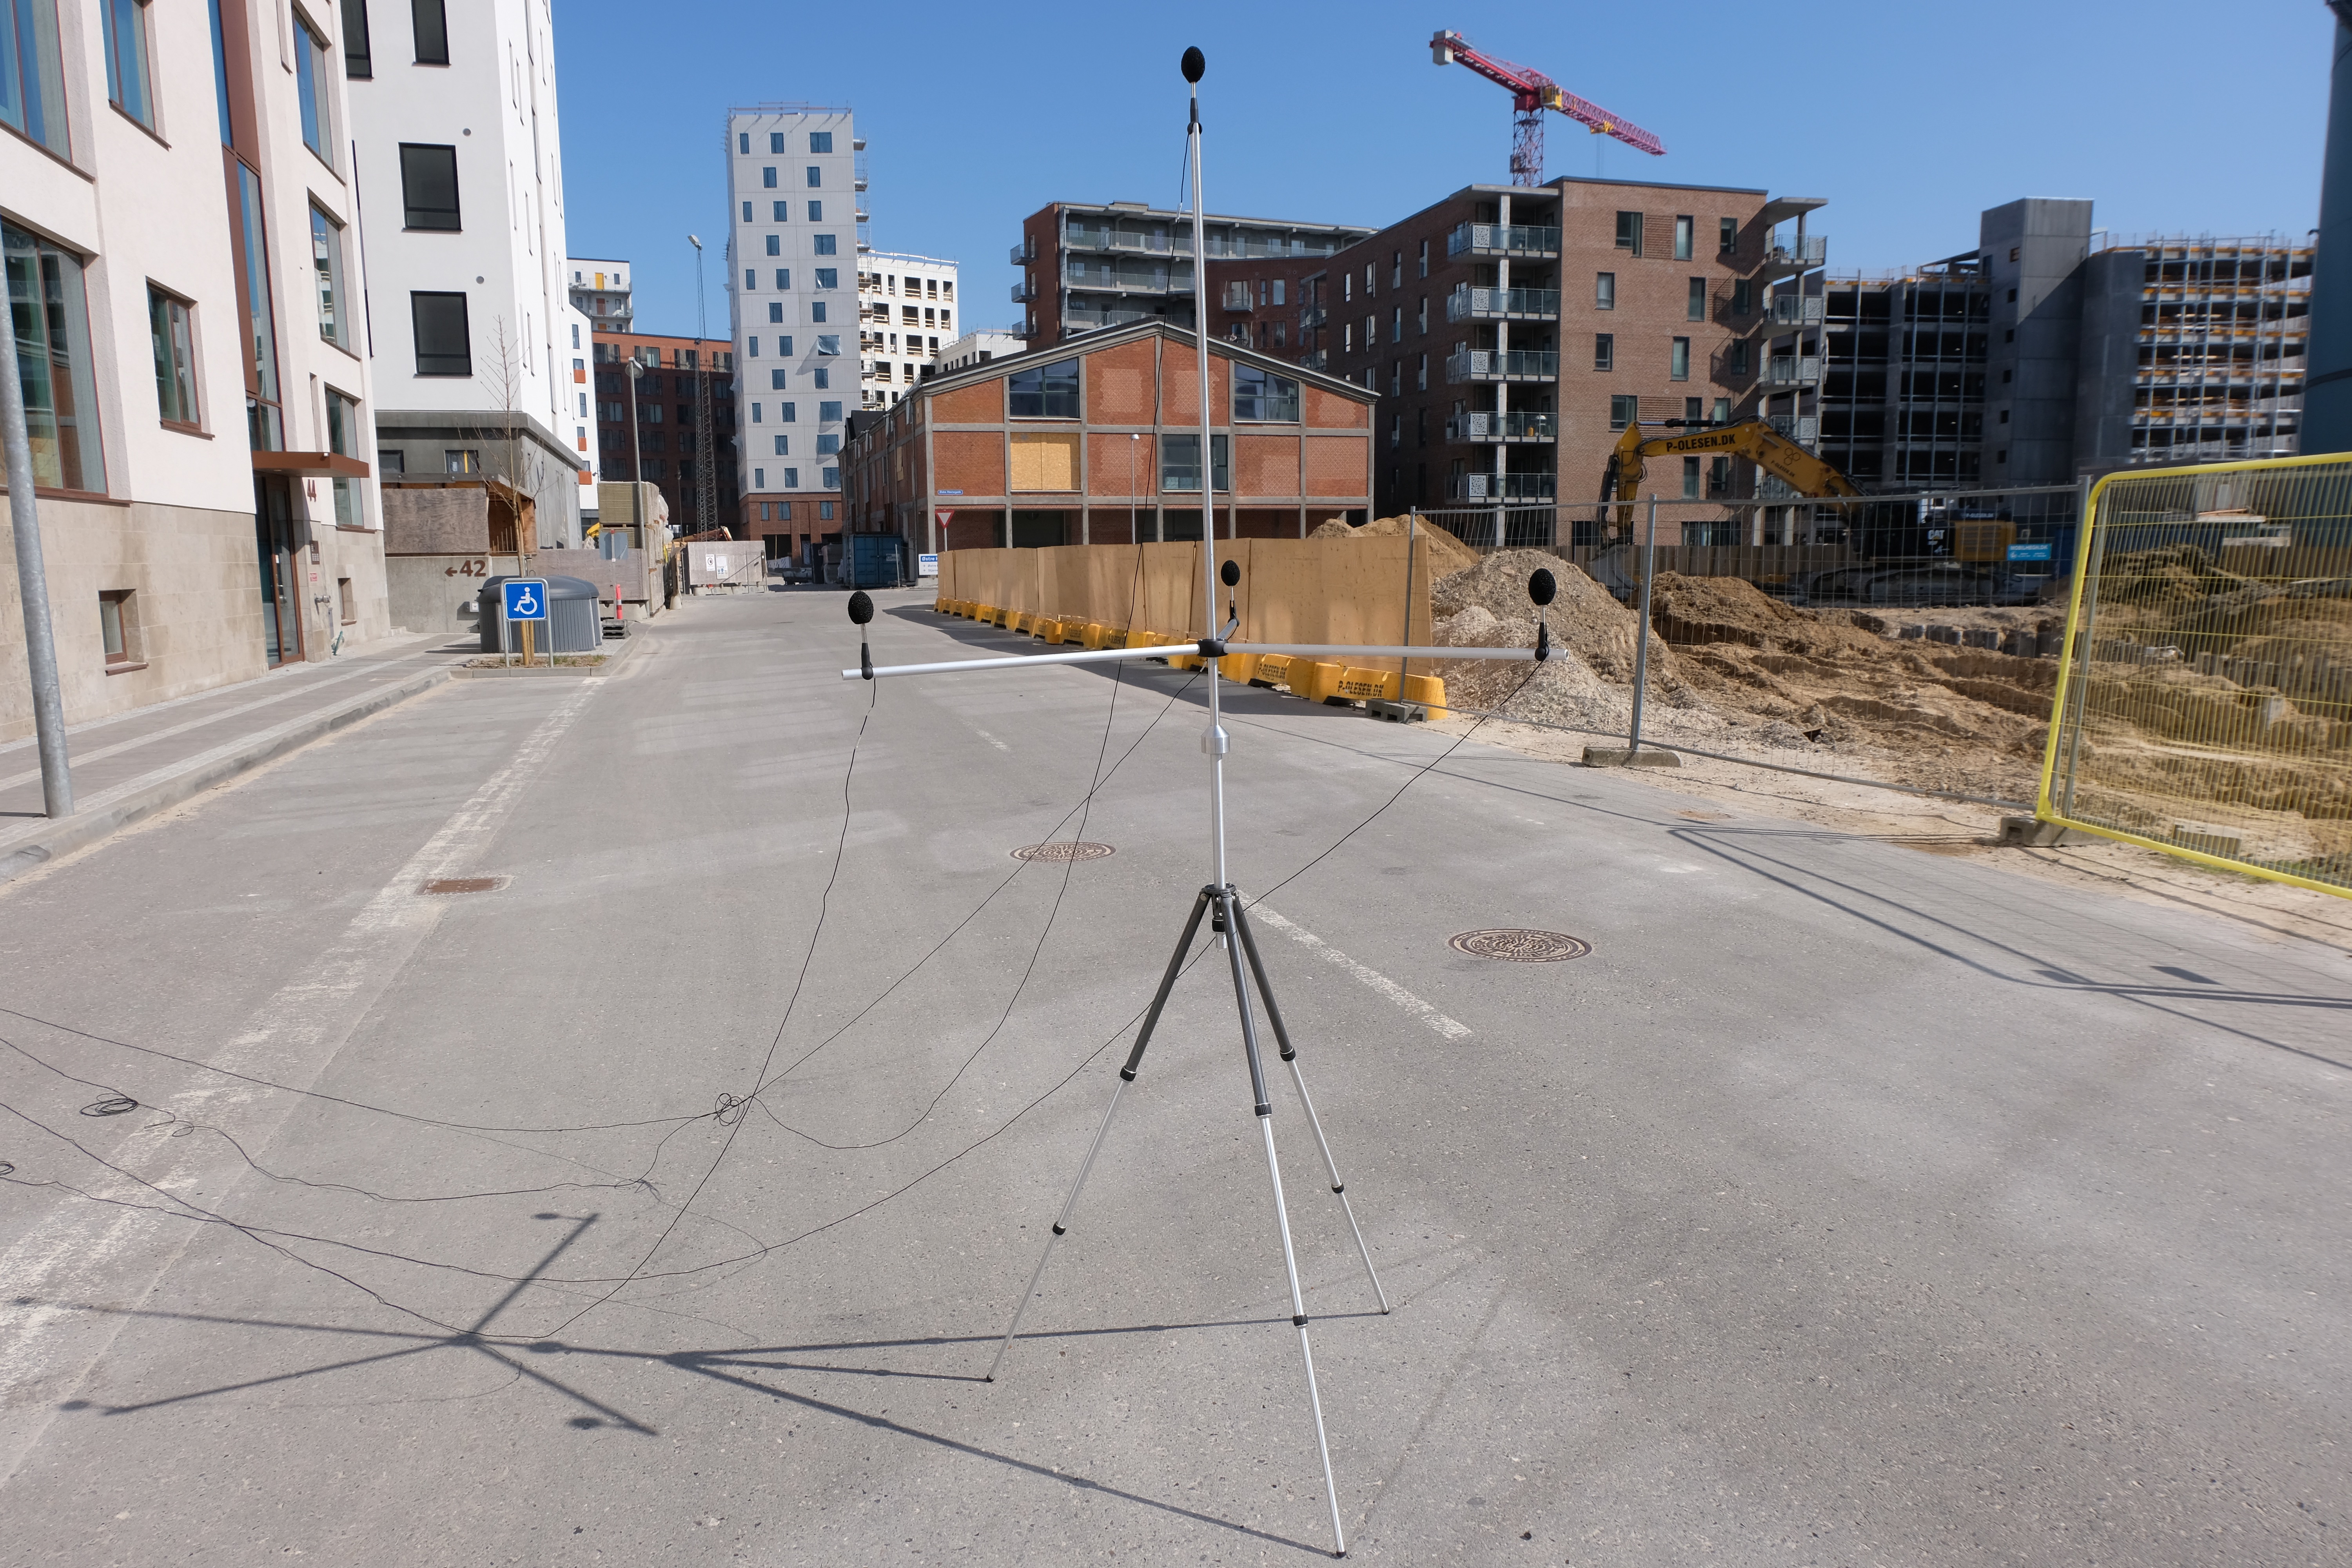
\includegraphics[width=0.7\textwidth]{Figures/micarraypic2.jpg}
    \caption{Prototype microphone array}
    \label{fig:micarraypic}
\end{figure}
